\documentclass{article}
\usepackage[T1]{fontenc}
\usepackage{lmodern}
\usepackage{graphicx}
\usepackage{amsmath,amssymb}
\usepackage[a4paper,margin=2cm]{geometry}
\usepackage[absolute,overlay]{textpos}
\setlength{\TPHorizModule}{1mm}
\setlength{\TPVertModule}{1mm}
\usepackage[indonesian]{babel}
\usepackage{hyperref}
\setlength{\emergencystretch}{2em}
% unit: Halaman 8

\begin{document}

% === Halaman 8 (llm) ===

\vspace{127.71mm}

Kriptografi mengenkripsi pesan sehingga maknanya tersamar
\vspace{20mm}

% deskripsi: Diagram proses enkripsi dan dekripsi yang menunjukkan perubahan dari plaintext 'Keamanan informasi' menjadi ciphertext '%j&g+9*4$\$jd8)?hyt8' melalui proses Enkripsi, dan sebaliknya melalui proses Dekripsi.
% bbox normalisasi: [0.1500, 0.2800, 0.8500, 0.7100]
\begin{textblock*}{147.00mm}(31.50mm,83.16mm)
\noindent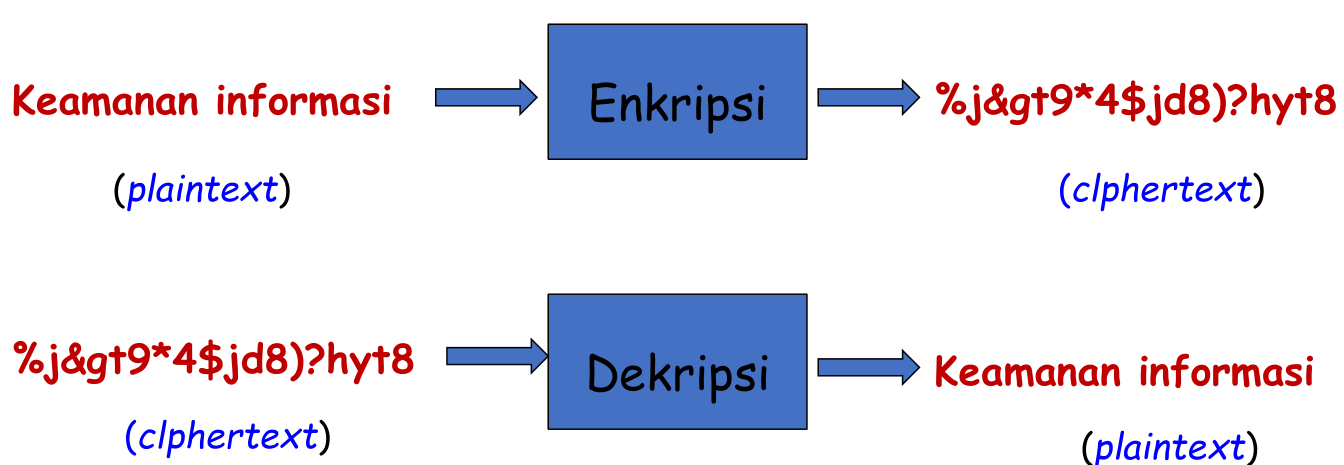
\includegraphics[width=147.00mm,height=127.71mm]{../../images/llm/page_008_img_01.png}%
\end{textblock*}

\end{document}
